\documentclass[a0paper,portrait]{baposter}
%%%%%%%%%%%%%%%%%%%%%%%%%%%%%%%%%%%%%%%%%%%%%%%%%%%%%%%%%%%%%%%%
% OU landscape  (a la place de portrait)
%%%%%%%%%%%%%%%%%%%%%%%%%%%%%%%%%%%%%%%%%%%%%%%%%%%%%%%%%%%%%%%%

%                     \documentclass[a0paper,portrait]{xebaposter}  
%                         ====> si baposter ne fonctionne pas sur MikeTeX


%%%%%% FORMAT EPISEN
%%%%%%%%%%%%%%%%%%%%%%%%%%%%%%%%%%%%%%%%%%%%%%%%%%%%%%%%%%%%%%%%
\usepackage{relsize}		% For \smaller
\usepackage{catchfile}
\usepackage{ifthen}
\CatchFileDef\TheLanguage{../language.tex}{\endlinechar=-1}
\ifthenelse{\equal{\TheLanguage}{french}}
 {
  \usepackage[french]{babel}
 }
 {
  \usepackage[english]{babel} 
 }
\usepackage{iflang}
\usepackage[utf8]{inputenc}
\usepackage[T1]{fontenc}
\usepackage{csquotes}
\usepackage[
 	natbib=true,
 	backend=biber,
 	style=alphabetic,
 	doi=false,
 	sorting=none,
 	sortcites
 ]{biblatex}
\addbibresource{../bibliographie.bib}
\AtBeginBibliography{\tiny}
\usepackage{lmodern}
\usepackage{xcolor}
\usepackage{stmaryrd}
\usepackage{amsmath}
\usepackage{amsfonts}
\usepackage{amssymb}
\usepackage{libertine}
\usepackage{caption}
\usepackage{subcaption}
\usepackage{float}
\usepackage{multirow}
\usepackage{apalike}
\usepackage{url}
\usepackage{tikz}
\usepackage{enumitem}
\usepackage{epigraph}
%\usetikzlibrary{shadows.blur}
\usepackage{lscape}
\usepackage{titletoc}
\usepackage{booktabs}
\usepackage{arydshln}
\usepackage{calc}
\usepackage[]{titlesec} 
\usepackage{fancyhdr}
\usepackage{lipsum}
\usepackage[]{todonotes}
\usepackage{url}
%\usepackage{minitoc}
\usepackage{listings}
\usepackage[lined,ruled,onelanguage,commentsnumbered,linesnumbered,inoutnumbered]{algorithm2e}
\CatchFileDef\TheManuscritTitle{../titre.tex}{\endlinechar=-1}
\CatchFileDef\TheAuthorEmail{../email.tex}{\endlinechar=-1}
\CatchFileDef\TheAuthorManuscript{../auteur.tex}{\endlinechar=-1}
\CatchFileDef\TheMemoireSubject{../sujet.tex}{\endlinechar=-1}
\CatchFileDef\TheMemoireKeywords{../keywords.tex}{\endlinechar=-1}

\newcommand{\departementEPISEN}{SI}    % write SI or ITS or ISBS

%%%%%%%%%%%%%%%%%%%%%%%%%%%%%%%%%%%%%%%%%%%%%%%%%%%%%%%%%%%%%%%%%%%%%%%%%%
%%%%%%%%%%%%%%%%%%%%%%%%%%%%%%%%%%%%%%%%%%%%%%%%%%%%%%%%%%%%%%%%%%%%%%%%%%
%%%%%%%%%%%%%%%%%%%%%%%%%%%%%%%%%%%%%%%%%%%%%%%%%%%%%%%%%%%%%%%%%%%%%%%%%%
%%%%%%%%%%%%%%%%%%%%%%%%%%%%%%%%%%%%%%%%%%%%%%%%%%%%%%%%%%%%%%%%%%%%%%%%%%
%
%  A PRIORI, NE PAS MODIFIER CE FICHIER !
%
%%%%%%%%%%%%%%%%%%%%%%%%%%%%%%%%%%%%%%%%%%%%%%%%%%%%%%%%%%%%%%%%%%%%%%%%%%
%%%%%%%%%%%%%%%%%%%%%%%%%%%%%%%%%%%%%%%%%%%%%%%%%%%%%%%%%%%%%%%%%%%%%%%%%%
%%%%%%%%%%%%%%%%%%%%%%%%%%%%%%%%%%%%%%%%%%%%%%%%%%%%%%%%%%%%%%%%%%%%%%%%%%
%%%%%%%%%%%%%%%%%%%%%%%%%%%%%%%%%%%%%%%%%%%%%%%%%%%%%%%%%%%%%%%%%%%%%%%%%%


%%%%%%%%%%%%%%%%%%%%%%%%%%%%%%%%%%%%%%%%%%%%%%%%%%%%%%%%%%%%%%%%%%%%%%%%%%
%%%%%%%%%%%%%%%%%%%%%%%%%%%%%%%%%%%%%%%%%%%%%%%%%%%%%%%%%%%%%%%%%%%%%%%%%%
% *********************** LES COULEURS (Départements) ********************
%%%%%%%%%%%%%%%%%%%%%%%%%%%%%%%%%%%%%%%%%%%%%%%%%%%%%%%%%%%%%%%%%%%%%%%%%%
%%%%%%%%%%%%%%%%%%%%%%%%%%%%%%%%%%%%%%%%%%%%%%%%%%%%%%%%%%%%%%%%%%%%%%%%%%

\definecolor{linkEpisenGris}{RGB}{81 98 111}
\definecolor{colorEPISEN-UPEC}{HTML}{4c6172}
%\definecolor{cadmiumred}{rgb}{0.89, 0.0, 0.13}
\definecolor{redUPEC}{HTML}{ef293d}

\ifthenelse{\equal{\departementEPISEN}{ITS}}
  {
   %%%%%%%%%%%%%%%%%%%%%%%%%%% POUR ITS
   \definecolor{colorEPISEN-MEMOIRE}{HTML}{655aa0}
   \definecolor{linkEpisenMEMOIRE}{RGB}{101 90 160}
   \definecolor{linkEpisenPoster}{RGB}{101 90 160}
   %\definecolor{linkEpisenPosterLight}{RGB}{223 221 238}
   %\definecolor{linkEpisenPosterLight}{HTML}{dfddee}
   \colorlet{linkEpisenPosterLight}{linkEpisenPoster!20}
   \colorlet{linkEpisenMemoireUltraLight}{linkEpisenPoster!7}
  }
  {
   \ifthenelse{\equal{\departementEPISEN}{SI}}
    {
	%%%%%%%%%%%%%%%%%%%%%%%%%%% POUR SI
	\definecolor{colorEPISEN-MEMOIRE}{HTML}{009fe3}
	\definecolor{linkEpisenMEMOIRE}{RGB}{0 159 227}
	\definecolor{linkEpisenPoster}{RGB}{0 159 227}
	%\definecolor{linkEpisenPosterLight}{RGB}{204 239 252}
  %\definecolor{linkEpisenPosterLight}{HTML}{cceffc}
  \colorlet{linkEpisenPosterLight}{linkEpisenPoster!20}
  \colorlet{linkEpisenMemoireUltraLight}{linkEpisenPoster!7}
    }
    {
	%%%%%%%%%%%%%%%%%%%%%%%%%%% POUR ISBS
	\definecolor{colorEPISEN-MEMOIRE}{HTML}{2fac66}
	\definecolor{linkEpisenMEMOIRE}{RGB}{47 172 102}
	\definecolor{linkEpisenPoster}{RGB}{47 172 102}
  %\definecolor{linkEpisenPosterLight}{RGB}{217 241 225}
  %\definecolor{linkEpisenPosterLight}{HTML}{d9f1e1}
  \colorlet{linkEpisenPosterLight}{linkEpisenPoster!20}
  \colorlet{linkEpisenMemoireUltraLight}{linkEpisenPoster!7}
    }
  }


%\definecolor{linkEpisenCyan}{RGB}{0 159 227}
%\definecolor{linkEpisenVert}{RGB}{47 172 102}
%\definecolor{linkEpisenViolet}{RGB}{101 90 160}
%\definecolor{colorEPISEN-SI}{HTML}{009fe3}
%\definecolor{colorEPISEN-ISBS}{HTML}{2fac66}
%\definecolor{colorEPISEN-ITS}{HTML}{655aa0}
%\definecolor{colorEPISEN-UPEC}{HTML}{4c6172}


%%%%%%%%%%%%%%%%%%%%%%%%%%%%%%%%%%%%%%%%%%%%%%%%%%%%%%%%%%%%%%%%%%%%%%%%%%
%%%%%%%%%%%%%%%%%%%%%%%%%%%%%%%%%%%%%%%%%%%%%%%%%%%%%%%%%%%%%%%%%%%%%%%%%%
%%%%%%%%%%%%%%%%%%%%%%%%%%%%%%%%%%%%%%%%%%%%%%%%%%%%%%%%%%%%%%%%%%%%%%%%%%
%%%%%%%%%%%%%%%%%%%%%%%%%%%%%%%%%%%%%%%%%%%%%%%%%%%%%%%%%%%%%%%%%%%%%%%%%%
%
%  VOUS POUVEZ APPORTER QUELQUES AJOUTS ICI
%
%%%%%%%%%%%%%%%%%%%%%%%%%%%%%%%%%%%%%%%%%%%%%%%%%%%%%%%%%%%%%%%%%%%%%%%%%%
%%%%%%%%%%%%%%%%%%%%%%%%%%%%%%%%%%%%%%%%%%%%%%%%%%%%%%%%%%%%%%%%%%%%%%%%%%
%%%%%%%%%%%%%%%%%%%%%%%%%%%%%%%%%%%%%%%%%%%%%%%%%%%%%%%%%%%%%%%%%%%%%%%%%%
%%%%%%%%%%%%%%%%%%%%%%%%%%%%%%%%%%%%%%%%%%%%%%%%%%%%%%%%%%%%%%%%%%%%%%%%%%

%%%%%%%%%%%%%%%%%%%%%%%%%%%%%%%%%%%%%%%%%%%%%%%%%%%%%%%%%%%%%%%%%%%%%%%%%%
%%% MODIFIER ICI pour les package tikz
%%%%%%%%%%%%%%%%%%%%%%%%%%%%%%%%%%%%%%%%%%%%%%%%%%%%%%%%%%%%%%%%%%%%%%%%%%
\usetikzlibrary{automata,positioning}
\AtBeginEnvironment{tikzpicture}{\tracinglostchars=0\relax}   % ==> pour éviter des warnings sur un nullfont

%%%%%%%%%%%%%%%%%%%%%%%%%%%%%%%%%%%%%%%%%%%%%%%%%%%%%%%%%%%%%%%%%%%%%%%%%%
%%% MODIFIER ICI POUR VOTRE PDF SI BESOIN
%%%%%%%%%%%%%%%%%%%%%%%%%%%%%%%%%%%%%%%%%%%%%%%%%%%%%%%%%%%%%%%%%%%%%%%%%%
\usepackage[colorlinks=true,bookmarks=false]{hyperref}
\AtBeginDocument{%
 \hypersetup{
   urlcolor=redUPEC,
   urlbordercolor=linkEpisenMEMOIRE,
   linkcolor=black,
   linkbordercolor=linkEpisenMEMOIRE,
   citecolor=linkEpisenMEMOIRE,
   citebordercolor=linkEpisenMEMOIRE,
   anchorcolor=linkEpisenMEMOIRE,
   pdftitle=\TheManuscritTitle,
   pdfauthor=\TheAuthorManuscript\\ (\TheAuthorEmail),
   pdfsubject=\TheMemoireSubject,
   pdfkeywords=\TheMemoireKeywords
}}


%%%%%%%%%%%%%%%%%%%%%%%%%%%%%%%%%%%%%%%%%%%%%%%%%%
%%% Setting Background Image 
%%%%%%%%%%%%%%%%%%%%%%%%%%%%%%%%%%%%%%%%%%%%%%%%%%
\background{
	\begin{tikzpicture}[remember picture,overlay]%
	\draw (current page.north west)+(-2em,2em) node[anchor=north west]
	{\includegraphics[height=1.1\textheight]{background}};
	\end{tikzpicture}
}

%%%%%%%%%%%%%%%%%%%%%%%%%%%%%%%%%%%%%%%%%%%%%%%%%%
%%% Utility functions 
%%%%%%%%%%%%%%%%%%%%%%%%%%%%%%%%%%%%%%%%%%%%%%%%%%

%%% Save space in lists. Use this after the opening of the list %%%%%%%%%%%%%%%%
\newcommand{\compresslist}{
	\setlength{\itemsep}{1pt}
	\setlength{\parskip}{0pt}
	\setlength{\parsep}{0pt}
}




%%%%%%%%%%%%%%%%%%%%%%%%%%%%%%%%%%%%%%%%%%%%%%%%%%%%%%%%%%%%%%%%%%%%%%%%%%
%%% Programme
%%%%%%%%%%%%%%%%%%%%%%%%%%%%%%%%%%%%%%%%%%%%%%%%%%%%%%%%%%%%%%%%%%%%%%%%%%


%%% Java
%%%%%%%%%%%%%%%%%%%%%%%%%%%%%%%%%%%%%%%%%%%%%%%%%%%%%%%%%%%%%%%%%%%%%%%%%%
\lstdefinestyle{myJava}{language=java, 
   keywordstyle=\bfseries\color{colorEPISEN-MEMOIRE},
   basicstyle=\normalfont,
   commentstyle=\color{linkEpisenGris},
   stringstyle=\color{brown},
   keepspaces=true, 
   numbers=left,
   numbersep=9pt,
   numberstyle=\tiny\color{linkEpisenGris},
   xleftmargin=20pt,
   framexleftmargin=1.77em,
   showstringspaces=true,
   showtabs=false,
   tabsize=2,
   breaklines=true,         % sets automatic line breaking
   breakatwhitespace=false, % sets if automatic breaks should only happen at whitespace
   columns=flexible,
   morekeywords={String, sealed, permits, System,out,println,-,+,*,/,++,--,<,>,=,!,!=},
   otherkeywords={\%*\%,+,!,!=,\&,<,>,=,++,--,\%/\%,\%\%},
   identifierstyle=\normalfont\itshape,
   literate=%
        {é}{{\'e}}1
        {è}{{\`e}}1
        {ê}{{\^e}}1
        {à}{{\`a}}1
        {â}{{\^a}}1
        {î}{{\^i}}1
        {ç}{{c}}1
        {ù}{{\`u}}1
      {|}{{$\hskip .001em\smash{\color{linkEpisenGris}\big|}\hskip .5em$}{ }}{1},
    mathescape=true,   
}

\lstnewenvironment{java}
   {\lstset{style=myJava}}
   {}

%%% R
%%%%%%%%%%%%%%%%%%%%%%%%%%%%%%%%%%%%%%%%%%%%%%%%%%%%%%%%%%%%%%%%%%%%%%%%%%
\lstdefinelanguage{R}{
   keywords={abbreviate,abline,abs,acos,acosh,action,add1,add,%
      aggregate,alias,Alias,alist,all,anova,any,aov,aperm,append,apply,%
      approx,approxfun,apropos,Arg,args,array,arrows,as,asin,asinh,%
      atan,atan2,atanh,attach,attr,attributes,autoload,autoloader,ave,%
      axis,backsolve,barplot,basename,besselI,besselJ,besselK,besselY,%
      beta,binomial,body,box,boxplot,break,browser,bug,builtins,bxp,by,%
      c,C,call,Call,case,cat,category,cbind,ceiling,character,char,%
      charmatch,check,chol,chol2inv,choose,chull,class,close,cm,codes,%
      coef,coefficients,co,col,colnames,colors,colours,commandArgs,%
      comment,complete,complex,conflicts,Conj,contents,contour,%
      contrasts,contr,control,helmert,contrib,convolve,cooks,coords,%
      distance,coplot,cor,cos,cosh,count,fields,cov,covratio,wt,CRAN,%
      create,crossprod,cummax,cummin,cumprod,cumsum,curve,cut,cycle,D,%
      data,dataentry,date,dbeta,dbinom,dcauchy,dchisq,de,debug,%
      debugger,Defunct,default,delay,delete,deltat,demo,de,density,%
      deparse,dependencies,Deprecated,deriv,description,detach,%
      dev2bitmap,dev,cur,deviance,off,prev,,dexp,df,dfbetas,dffits,%
      dgamma,dgeom,dget,dhyper,diag,diff,digamma,dim,dimnames,dir,%
      dirname,dlnorm,dlogis,dnbinom,dnchisq,dnorm,do,dotplot,double,%
      download,dpois,dput,drop,drop1,dsignrank,dt,dummy,dump,dunif,%
      duplicated,dweibull,dwilcox,dyn,edit,eff,effects,eigen,else,%
      emacs,end,environment,env,erase,eval,equal,evalq,example,exists,%
      exit,exp,expand,expression,External,extract,extractAIC,factor,%
      fail,family,fft,file,filled,find,fitted,fivenum,fix,floor,for,%
      For,formals,format,formatC,formula,Fortran,forwardsolve,frame,%
      frequency,ftable,ftable2table,function,gamma,Gamma,gammaCody,%
      gaussian,gc,gcinfo,gctorture,get,getenv,geterrmessage,getOption,%
      getwd,gl,glm,globalenv,gnome,GNOME,graphics,gray,grep,grey,grid,%
      gsub,hasTsp,hat,heat,help,hist,home,hsv,httpclient,I,identify,if,%
      ifelse,Im,image,\%in\%,index,influence,measures,inherits,install,%
      installed,integer,interaction,interactive,Internal,intersect,%
      inverse,invisible,IQR,is,jitter,kappa,kronecker,labels,lapply,%
      layout,lbeta,lchoose,lcm,legend,length,levels,lgamma,library,%
      licence,license,lines,list,lm,load,local,locator,log,log10,log1p,%
      log2,logical,loglin,lower,lowess,ls,lsfit,lsf,ls,machine,Machine,%
      mad,mahalanobis,make,link,margin,match,Math,matlines,mat,matplot,%
      matpoints,matrix,max,mean,median,memory,menu,merge,methods,min,%
      missing,Mod,mode,model,response,mosaicplot,mtext,mvfft,na,nan,%
      names,omit,nargs,nchar,ncol,NCOL,new,next,NextMethod,nextn,%
      nlevels,nlm,noquote,NotYetImplemented,NotYetUsed,nrow,NROW,null,%
      numeric,\%o\%,objects,offset,old,on,Ops,optim,optimise,optimize,%
      options,or,order,ordered,outer,package,packages,page,pairlist,%
      pairs,palette,panel,par,parent,parse,paste,path,pbeta,pbinom,%
      pcauchy,pchisq,pentagamma,persp,pexp,pf,pgamma,pgeom,phyper,pico,%
      pictex,piechart,Platform,plnorm,plogis,plot,pmatch,pmax,pmin,%
      pnbinom,pnchisq,pnorm,points,poisson,poly,polygon,polyroot,pos,%
      postscript,power,ppoints,ppois,predict,preplot,pretty,Primitive,%
      print,prmatrix,proc,prod,profile,proj,prompt,prop,provide,%
      psignrank,ps,pt,ptukey,punif,pweibull,pwilcox,q,qbeta,qbinom,%
      qcauchy,qchisq,qexp,qf,qgamma,qgeom,qhyper,qlnorm,qlogis,qnbinom,%
      qnchisq,qnorm,qpois,qqline,qqnorm,qqplot,qr,Q,qty,qy,qsignrank,%
      qt,qtukey,quantile,quasi,quit,qunif,quote,qweibull,qwilcox,%
      rainbow,range,rank,rbeta,rbind,rbinom,rcauchy,rchisq,Re,read,csv,%
      csv2,fwf,readline,socket,real,Recall,rect,reformulate,regexpr,%
      relevel,remove,rep,repeat,replace,replications,report,require,%
      resid,residuals,restart,return,rev,rexp,rf,rgamma,rgb,rgeom,R,%
      rhyper,rle,rlnorm,rlogis,rm,rnbinom,RNGkind,rnorm,round,row,%
      rownames,rowsum,rpois,rsignrank,rstandard,rstudent,rt,rug,runif,%
      rweibull,rwilcox,sample,sapply,save,scale,scan,scan,screen,sd,se,%
      search,searchpaths,segments,seq,sequence,setdiff,setequal,set,%
      setwd,show,sign,signif,sin,single,sinh,sink,solve,sort,source,%
      spline,splinefun,split,sqrt,stars,start,stat,stem,step,stop,%
      storage,strstrheight,stripplot,strsplit,structure,strwidth,sub,%
      subset,substitute,substr,substring,sum,summary,sunflowerplot,svd,%
      sweep,switch,symbol,symbols,symnum,sys,status,system,t,table,%
      tabulate,tan,tanh,tapply,tempfile,terms,terrain,tetragamma,text,%
      time,title,topo,trace,traceback,transform,tri,trigamma,trunc,try,%
      ts,tsp,typeof,unclass,undebug,undoc,union,unique,uniroot,unix,%
      unlink,unlist,unname,untrace,update,upper,url,UseMethod,var,%
      variable,vector,Version,vi,warning,warnings,weighted,weights,%
      which,while,window,write,\%x\%,x11,X11,xedit,xemacs,xinch,xor,%
      xpdrows,xy,xyinch,yinch,zapsmall,zip},
   otherkeywords={0,1,2,3,4,5,6,7,8,9},
   morekeywords={TRUE,FALSE,for,if,then,else,function,in},
   otherkeywords={-,+,!,!=,<,>,~,$,*,\&,\%/\%,\%*\%,\%\%,_,/},%
   alsoother={._$},%
   sensitive,%
   morecomment=[l]{\#},%
   morestring=[d]",%
   morestring=[d]',
   literate=%
        {é}{{\'e}}1
        {è}{{\`e}}1
        {ê}{{\^e}}1
        {à}{{\`a}}1
        {â}{{\^a}}1
        {î}{{\^i}}1
        {ç}{{c}}1
        {ù}{{\`u}}1
        {|}{{$\hskip .001em\smash{\color{linkEpisenGris}\big|}\hskip .5em$}{ }}{1},
}

\lstdefinestyle{myR}{
   language=R,
   keywordstyle=\bfseries\color{colorEPISEN-MEMOIRE},
   basicstyle=\normalfont,
   stringstyle=\color{brown},
   commentstyle=\color{linkEpisenGris},
   keepspaces=true, 
   numbers=left,
   numbersep=9pt,
   numberstyle=\tiny\color{linkEpisenGris},
   xleftmargin=20pt,
   framexleftmargin=1.5em,
   showstringspaces=true,
   tabsize=2,
   breaklines=true,         % sets automatic line breaking
   breakatwhitespace=false, % sets if automatic breaks should only happen at whitespace
   columns=flexible,
   escapeinside={\%*}{*)},
   identifierstyle=\normalfont\itshape,
} 

\lstnewenvironment{R}
    {\lstset{style=myR}}
    {}

%%% Python
%%%%%%%%%%%%%%%%%%%%%%%%%%%%%%%%%%%%%%%%%%%%%%%%%%%%%%%%%%%%%%%%%%%%%%%%%%

\lstdefinestyle{myPython}{language=python, 
   keywordstyle=\bfseries\color{colorEPISEN-MEMOIRE},
   basicstyle=\normalfont,
   commentstyle=\color{linkEpisenGris},
   stringstyle=\color{brown},
   keepspaces=true, 
   numbers=left,
   numbersep=9pt,
   numberstyle=\tiny\color{linkEpisenGris},
   xleftmargin=20pt,
   framexleftmargin=1.5em,
   showstringspaces=true,
   showtabs=false,
   tabsize=2,
   breaklines=true,         % sets automatic line breaking
   breakatwhitespace=false, % sets if automatic breaks should only happen at whitespace
   columns=flexible,
   morekeywords={-,+,*,/,++,--,<,>,=,!,!=},
   otherkeywords={\%*\%,+,!,!=,\&,<,>,=,\%/\%,\%\%},
   identifierstyle=\normalfont\itshape,
   literate=%
        {é}{{\'e}}1
        {è}{{\`e}}1
        {ê}{{\^e}}1
        {à}{{\`a}}1
        {â}{{\^a}}1
        {î}{{\^i}}1
        {ç}{{c}}1
        {ù}{{\`u}}1
        {|}{{$\hskip .001em\smash{\color{linkEpisenGris}\big|}\hskip .5em$}{ }}{1},
    mathescape=true,
%  frame=single,
%  framesep=\fboxsep,
%  framerule=1pt,
%  rulecolor=\color{colorEPISEN-MEMOIRE},
%  xleftmargin=\dimexpr\fboxsep+\fboxrule\relax,
%  xrightmargin=\dimexpr\fboxsep+\fboxrule\relax
%  frame=lines
}

\lstnewenvironment{python}
   {\lstset{style=myPython}}
   {}


%%% Algorithmes
%%%%%%%%%%%%%%%%%%%%%%%%%%%%%%%%%%%%%%%%%%%%%%%%%%%%%%%%%%%%%%%%%%%%%%%%%%

%https://tex.stackexchange.com/questions/668747/different-color-for-algorithm2e-keywords
\renewcommand{\KwSty}[1]{\textnormal{\textcolor{colorEPISEN-MEMOIRE}{\bfseries #1}}\unskip}


% ****************
% Pour les autres langages, débrouillez vous un peu !!!
% ****************



%%%%%%%%%%%%%%%%%%%%%%%%%%%%%%%%%%%%%%%%%%%%%%%%%%%%%%%%%%%%%%%%%%%%%%%%%%
%%%%%%%%%%%%%%%%%%%%%%%%%%%%%%%%%%%%%%%%%%%%%%%%%%%%%%%%%%%%%%%%%%%%%%%%%%
%%%%%%%%%%%%%%%%%%%%%%%%%%%%%%%%%%%%%%%%%%%%%%%%%%%%%%%%%%%%%%%%%%%%%%%%%%
%%%%%%%%%%%%%%%%%%%%%%%%%%%%%%%%%%%%%%%%%%%%%%%%%%%%%%%%%%%%%%%%%%%%%%%%%%
%
%  A PRIORI, NE PLUS MODIFIER LA SUITE DE CE FICHIER !
%
%%%%%%%%%%%%%%%%%%%%%%%%%%%%%%%%%%%%%%%%%%%%%%%%%%%%%%%%%%%%%%%%%%%%%%%%%%
%%%%%%%%%%%%%%%%%%%%%%%%%%%%%%%%%%%%%%%%%%%%%%%%%%%%%%%%%%%%%%%%%%%%%%%%%%
%%%%%%%%%%%%%%%%%%%%%%%%%%%%%%%%%%%%%%%%%%%%%%%%%%%%%%%%%%%%%%%%%%%%%%%%%%
%%%%%%%%%%%%%%%%%%%%%%%%%%%%%%%%%%%%%%%%%%%%%%%%%%%%%%%%%%%%%%%%%%%%%%%%%%


\ifthenelse{\equal{\TheLanguage}{french}}
 {
  \DefineBibliographyStrings{french}{%
      backrefpage = {cf. page},
      backrefpages = {cf. pages},
      urlseen = {\textsc{url}~:},
      urlfrom = {\textsc{url}~:},
      in={dans},
      volume={vol\adddot},
      pages = {pp\adddot},
      byeditor = {Dir\adddot\space}
  }
  \DefineBibliographyExtras{french}{\protected\def\bibrangedash{--}}
 }
 {
  \DefineBibliographyStrings{english}{%
      backrefpage = {see page},
      backrefpages = {see pages},
      urlseen = {\textsc{url}:},
      urlfrom = {\textsc{url}:},
      byeditor = {Ed\adddot\space}
  }
 }
\DeclareFieldFormat{url}{\bibstring{urlfrom}\addcolon\space\url{#1}}

\usepackage{xpatch}
% No dot before number of articles
\xpatchbibmacro{volume+number+eid}{%
  \setunit*{\adddot}%
}{%
}{}{}


% Comma before and after journal volume
\renewbibmacro*{volume+number+eid}{%
  \setunit*{\addcomma\space}% NEW
  \printfield{volume}%
%  \setunit*{\adddot}% DELETED
  \setunit*{\addcomma\space}% NEW
  \printfield{number}%
  \setunit{\addcomma\space}%
  \printfield{eid}}

% Prefixes for journal volume and number
\DeclareFieldFormat[article]{volume}{\bibstring{volume}~#1}% volume of a journal
\DeclareFieldFormat[article]{number}{\bibstring{number}~#1,}% number of a journal


\newtoggle{bbx:datemissing}

\renewbibmacro*{date}{\toggletrue{bbx:datemissing}%
}

\renewbibmacro*{issue+date}{%
  \toggletrue{bbx:datemissing}%
  \iffieldundef{issue}
    {}
    {\printtext[parens]{%
       \printfield{issue}}}%
  \newunit}

\newbibmacro*{date:print}{%
  \togglefalse{bbx:datemissing}%
  \printdate}

\renewbibmacro*{chapter+pages}{%
  \printfield{chapter}%
  \setunit{\bibpagespunct}%
  \printfield{pages}%
  \newunit
  \setunit*{\addcomma\space}
  \usebibmacro{date:print}%
  \newunit}

\renewbibmacro*{note+pages}{%
  \printfield{note}%
  \setunit{\bibpagespunct}%
  \printfield{pages}%
  \newunit
  \setunit*{\addcomma\space}
  \usebibmacro{date:print}%
  \newunit}

\renewbibmacro*{addendum+pubstate}{%
  \iftoggle{bbx:datemissing}
    {\usebibmacro{date:print}}
    {}%
  \printfield{addendum}%
  \newunit\newblock
  \printfield{pubstate}}


\begin{document}


%%% Configuration du poster
%%%%%%%%%%%%%%%%%%%%%%%%%%%%%%%%%%%%%%%%%%%%%%%%%%%%%%%%%%%%%%%%
\begin{poster}{
%%%%%%%%%%%%%%%%%%%%%%%%%%%%%%%%%%%%%%%%%%%%%%%%%%%%%%%%%%%%%%%%
% METTRE TRUE pour GRID pour visualiser le placement des boites
%%%%%%%%%%%%%%%%%%%%%%%%%%%%%%%%%%%%%%%%%%%%%%%%%%%%%%%%%%%%%%%%    
	grid=false,
	borderColor=linkEpisenGris,
	headerColorOne=linkEpisenPoster,
	headerColorTwo=linkEpisenPosterLight,
	headerFontColor=black,
	boxColorOne=linkEpisenPosterLight,
	textborder=rectangle,
	bgColorOne=linkEpisenPoster,
	bgColorTwo=linkEpisenMemoireUltraLight,
	headerborder=open,
    boxshade=plain,
	background=shadetb,
	textfont=\large,   
	headerfont=\LARGE\sf\bf,
}
%%% Eye Cacther %%%%%%%%%%%%%%%%%%%%%%%%%%%%%%%%%%%%%%%%%%%%%%%%%%%%%%%%%%%%%%%
{%unused
}
{
%%%%%%%%%%%%%%%%%%%%%%%%%%%%%%%%%%%%%%%%%%%%%%%%%%%%%%%%%%%%%%%%
%Titre du memoire
%%%%%%%%%%%%%%%%%%%%%%%%%%%%%%%%%%%%%%%%%%%%%%%%%%%%%%%%%%%%%%%%
\sf\bf \TheManuscritTitle
}
%%%%%%%%%%%%%%%%%%%%%%%%%%%%%%%%%%%%%%%%%%%%%%%%%%%%%%%%%%%%%%%%
% Authors
%%%%%%%%%%%%%%%%%%%%%%%%%%%%%%%%%%%%%%%%%%%%%%%%%%%%%%%%%%%%%%%%
{
	\vspace{1em} \TheAuthorManuscript\\
	{\smaller \url{\TheAuthorEmail}}
}
%%%%%%%%%%%%%%%%%%%%%%%%%%%%%%%%%%%%%%%%%%%%%%%%%%%%%%%%%%%%%%%%
% Logo
%%%%%%%%%%%%%%%%%%%%%%%%%%%%%%%%%%%%%%%%%%%%%%%%%%%%%%%%%%%%%%%%
{
	\begin{tabular}{c@{\hskip 2.8cm}c@{\hskip -1.3cm}c}
		\ifthenelse{\equal{\departementEPISEN}{ITS}}
			{
	 		    %%%%%%%%%%%%%%%%%%%%%%%%%%% POUR ITS
					\begin{minipage}[c][-8ex][b]{0em}
					
\includegraphics[height=2.2cm]{../images/logos/upec-blanc-sans-baseline.png} 
					\end{minipage} &
					
\includegraphics[height=3cm]{../images/logos/EPISEN_logo-ITS-blanc-POSTER.png} &
					
\includegraphics[height=2.3cm]{../images/logos/entrepriseLogo.png}\\
			}
			{
				\ifthenelse{\equal{\departementEPISEN}{SI}}
    			{
					%%%%%%%%%%%%%%%%%%%%%%%%%%% POUR SI
					\begin{minipage}[c][-8ex][b]{0em}
					
\includegraphics[height=2.2cm]{../images/logos/upec-blanc-sans-baseline.png} 
					\end{minipage} &
					
\includegraphics[height=3cm]{../images/logos/EPISEN_logo-SI-blanc-POSTER.png} &
					
\includegraphics[height=2.3cm]{../images/logos/entrepriseLogo.png}\\
    			}
				{
					%%%%%%%%%%%%%%%%%%%%%%%%%%% POUR ISBS
					\begin{minipage}[c][-8ex][b]{0em}
					
\includegraphics[height=2.2cm]{../images/logos/upec-blanc-sans-baseline.png} 
					\end{minipage} &
					
\includegraphics[height=3cm]{../images/logos/EPISEN_logo-ISBS-blanc-POSTER.png} &
					
\includegraphics[height=2.3cm]{../images/logos/entrepriseLogo.png}\\
				}
	    	}
	\end{tabular}
}



%%%%%%%%%%%%%%%%%%%%%%%%%%%%%%%%%%%%%%%%%%%%%%%%%%%%%%%%%%%%%%%%
%%%%%%%%%%%%%%%%%%%%%%%%%%%%%%%%%%%%%%%%%%%%%%%%%%%%%%%%%%%%%%%%
% Ici le debut de vos boites !
%%%%%%%%%%%%%%%%%%%%%%%%%%%%%%%%%%%%%%%%%%%%%%%%%%%%%%%%%%%%%%%%
%%%%%%%%%%%%%%%%%%%%%%%%%%%%%%%%%%%%%%%%%%%%%%%%%%%%%%%%%%%%%%%%

\begin{posterbox}[name=problematique,span=3,column=0,row=0]{Problématique}
On parle ici du problème en général. On peut rajouter une petite figure. Ici la boîte est sur les 2 colonnes. Elle s'appele ``problematique'' et on peut définir à quelle colonne et ligne elle appartient dans la grille du poster. Ceci est bien sûr qu'un exemple, vous pouvez mettre la première boîte que sur une unique colonne.
\begin{center}
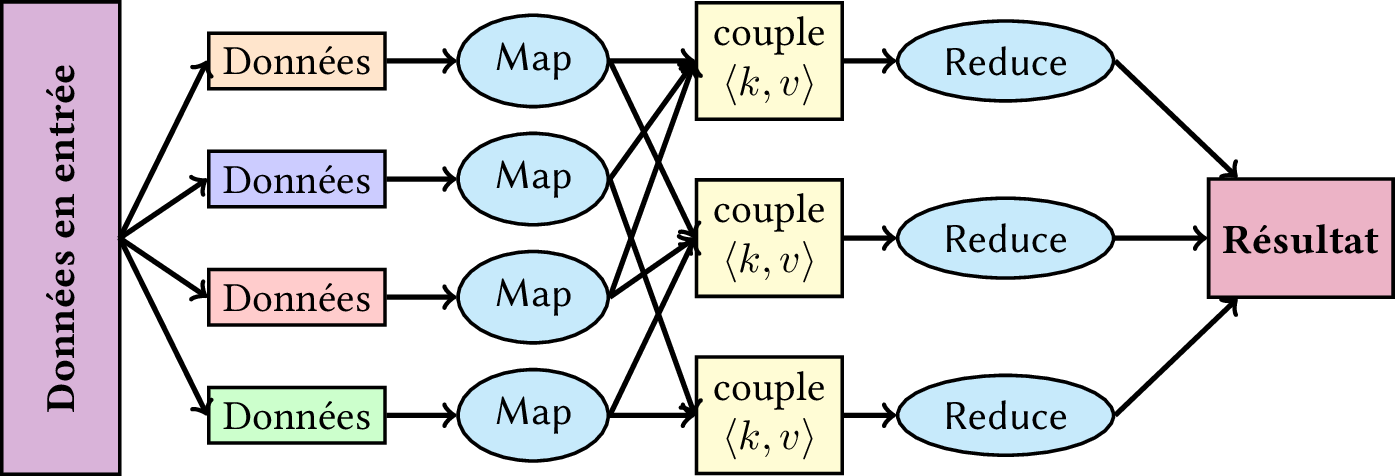
\includegraphics[height=3cm]{../images/Mapreduce.png}
\end{center}
\end{posterbox}

\begin{posterbox}[name=important,column=1,below=problematique]{Points importants}
Ici ~; les mêmes points que dans le mémoire car provenant du même fichier~:
\begin{itemize}
	\item Citer vos sources~;
	\item Référencer les figures dans le texte~;
	\item Avoir une notation cohérente entre les différents supports~;
	\item Respecter le typographie pour le bien être du relecteur.
\end{itemize}

\end{posterbox}

\begin{posterbox}[name=formule,span=1,column=2,below=problematique]{Formule importante}
Ici, LA formule qui est à la base de tout votre mémoire. Exemple~:
\input{../ShareText/maths1.tex}
Bien sûr, on peux mettre aussi un algo ou un design de programme ou un protocol ou essai clinique {\it etc.}
\end{posterbox}

\begin{posterbox}[name=tableau,span=2,column=1,below=formule]{Tableau important}
Ici les données les plus importants de votre travail, identiques à celles de votre mémoire~: 
\begin{center}
\begin{tabular}{|l|l|l|}
\hline
Département & Nombre de chaises & Nombre de prises électriques\\
\hline
\hline
ITS & 150 & 20\\
\hline
SI & 149 & 25 \\
\hline
ISBS & 151 & 19\\
\hline
\end{tabular}
\end{center}
Sur 2 colonnes car le tableau est un peu gros. Vous trouverez sur le net comment faire
des tableaux bien plus jolies que cela. Exemples~: \url{https://fr.overleaf.com/learn/latex/Tables}

Ici, je rajoute du test pour la bibliographie (références)~:
\begin{itemize}
\item Un article de revue \cite{ref1}~;
\item Article de Conférence \cite{ref3}~;
\item Un livre \cite{ref4}
\end{itemize}
\end{posterbox}


\begin{posterbox}[name=graph,span=1,column=0,below=problematique]{Un graphe}
Une autre image~:
\begin{center}
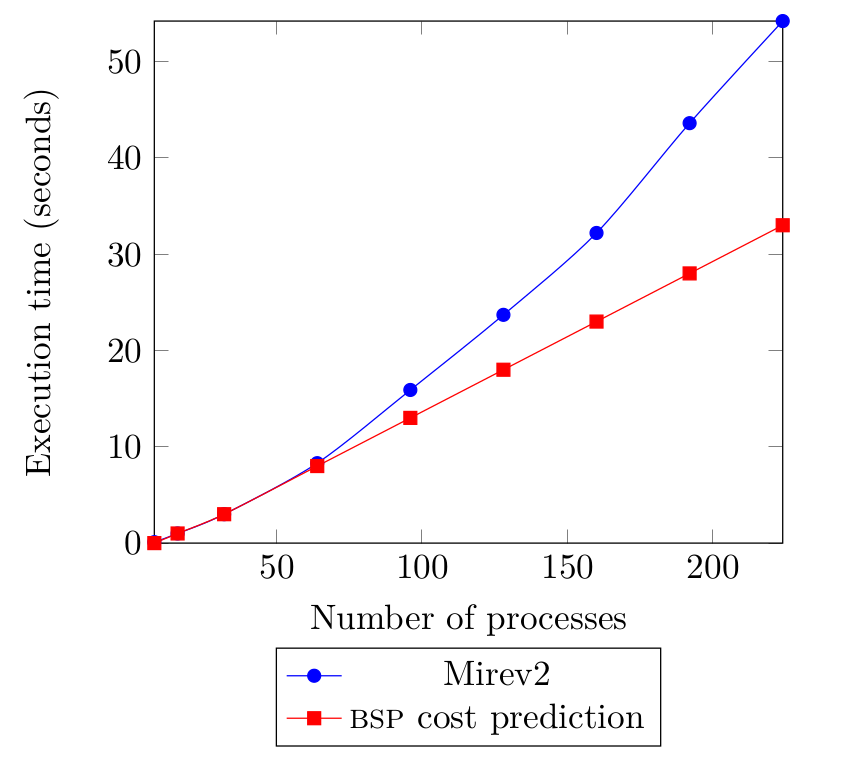
\includegraphics[height=5cm]{../images/reality.png}
\end{center}
\end{posterbox}


%%%%%%%%%%%%%%%%%%%%%%%%%%%%%%%%%%%%%%%%%%%%%%%%%%%%%%%%%%%%%%%%
%%% Remerciements et bibliographie
%%%%%%%%%%%%%%%%%%%%%%%%%%%%%%%%%%%%%%%%%%%%%%%%%%%%%%%%%%%%%%%%
\ifthenelse{\equal{\TheLanguage}{french}}{
   \begin{posterbox}[name=acknowledgements,column=2,above=bottom]{Remerciements}}
  {\begin{posterbox}[name=acknowledgements,column=2,above=bottom]{Acknowledgements}}
 \smaller						
 \vspace{-0.4em}			% Save some space at the beginning
Ce travail a été effectué avec le soutien de l'EPISEN. Je remercie mon chat, l'EPISEN,
Gandalf et toute la communauté de l'anneau.
\end{posterbox}

\ifthenelse{\equal{\TheLanguage}{french}}{
   \begin{posterbox}[name=references,column=2,row=0.78]{Références}}
  {\begin{posterbox}[name=references,column=2,row=0.78]{References}}

\relsize{-5}
\vspace{-0.4em}
\setlength{\baselineskip}{0.4em}
\itemsep=-0.01em
\renewcommand{\section}[2]{\vskip 0.05em}
\printbibliography
\end{posterbox}

 \begin{posterbox}[name=code,span=1,column=0,below=tableau]{Un code Java}
Un exemple de code Java~:
\begin{footnotesize}
\begin{java}
public class {
|	...
|	public static void main(String arg){
|	|	System.out.println("sdmklfjsdfj dfsdf ");
|	|	/* A loop et avec des maths $x=\int_{i=1}^n \sin{x}$ */
|	|	for(int i=0;i<n;i++)
|	|	|	if (1=1)
|	|	|	|	Toto.add(i)
|	}
}
\end{java}
\end{footnotesize}
\end{posterbox}




%%%%%%%%%%%%%%%%%%%%%%%%%%%%%%%%%%%%%%%%%%%%%%%%%%%%%%%%%%%%%%%%
%%%%%%%%%%%%%%%%%%%%%%%%%%%%%%%%%%%%%%%%%%%%%%%%%%%%%%%%%%%%%%%%
% Ici ce termine la déclaration de vos boites !
% Ne plus rien mettre après !
%%%%%%%%%%%%%%%%%%%%%%%%%%%%%%%%%%%%%%%%%%%%%%%%%%%%%%%%%%%%%%%%
%%%%%%%%%%%%%%%%%%%%%%%%%%%%%%%%%%%%%%%%%%%%%%%%%%%%%%%%%%%%%%%%
\end{poster}





\end{document}
